\chapter{Koncepcja rozwiązania}
\label{chapter:requirements}

W ramach rozdziału omówiono założenia projektowe oraz koncepcję platformy.
Pierwszy podrozdział opisuje sposób testowania wybrany do weryfikacji programów studentów w ramach narzędzia.
W kolejnych podrozdziałach omówiono organizację pracy dla projektu informatycznego oraz przedstawiono problemy, na jakie napotykają prowadzący i~studenci podczas uczestnictwa w takim zadaniu.
Dla każdej z wymienionych trudności opisano sposób jej załagodzenia z wykorzystaniem zaprojektowanej w ramach pracy platformy.
W przedostatniej sekcji omówiono wymagania niefunkcjonalne dla narzędzia.
Ostatni podrozdział zawiera opis ograniczeń proponowanego rozwiązania.

\section{Testy akceptacyjne jako narzędzie weryfikacji}

W celu oceny poprawności działania programów studentów należy przeprowadzić odpowiednie testy.
Jedną z kategorii podziału testów, jest klasyfikacja ze względu na wiedzę na temat testowanego programu.
W tym przypadku wyróżniamy dwie podstawowe kategorie:
\begin{itemize}
    \item testy czarnej skrzynki (ang. black box testing),
    \item testy białej skrzynki (ang. white box testing).
\end{itemize}

\begin{figure}[h]
    \centering
    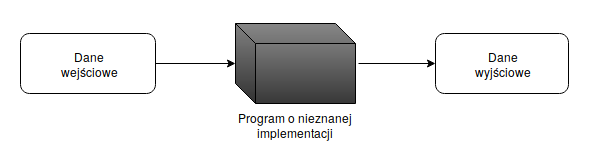
\includegraphics[width = 13cm]{chapter02/black-box.png}
    \caption{Schemat testu czarnej skrzynki.}
    \label{fig:black-box}
\end{figure}

Na rysunku \ref{fig:black-box} został przedstawiony ogólny schemat procesu dla black box testów.
Dla tego przypadku fragment kodu lub cały testowany program nie jest znany dla testera.
Black box testing może odnosić się zarówno do testów funkcjonalnych, jak i niefunkcjonalnych.
Najczęściej jednak dotyczy on pierwszego rodzaju.
Testy czarnej skrzynki mają zastosowanie na następujących poziomach:
\begin{itemize}
    \item testów integracyjnych,
    \item testów systemowych,
    \item testów akceptacyjnych.
\end{itemize}

Ten rodzaj testów jest wykonywany z perspektywy użytkownika.
Pozwala to między innymi na wskazanie rozbieżności pomiędzy wytworzonym kodem a założoną specyfikacją zadania w tym:
\begin {itemize}
    \item niepoprawnych lub brakujących funkcjonalności,
    \item błędów w interfejsie,
    \item błędów w strukturach danych,
    \item błędów zachowania programów oraz wydajnościowych.
\end{itemize}
Zaletą tego rodzaju podejścia jest fakt, że osoba testująca nie musi znać kodu oraz języka programowania, w którym została napisana aplikacja.

\begin{figure}[h]
    \centering
    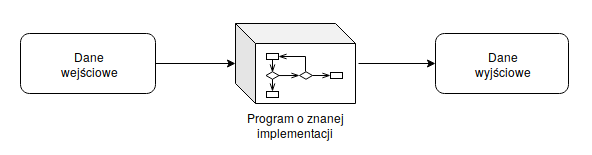
\includegraphics[width = 13cm]{chapter02/white-box.png}
    \caption{Schemat testu białej skrzynki.}
    \label{fig:white-box}
\end{figure}

Drugim rodzajem testowania programów jest metoda białej skrzynki (ang. white box testing).
Schemat procesu tego typu został przedstawiony na rysunku \ref{fig:white-box}.
W tym przypadku tester zna pełną implementację badanej funkcjonalności.
Jego zadaniem jest dobranie odpowiednich wartości wejściowych dla sprawdzanej funkcjonalności i uzyskanie założonych wartości wyjściowych, w ramach testowanego kodu.
Do realizacji tego zadania niezbędne są umiejętności programistyczne i wiedza na temat implementacji.
Testy białej skrzynki mają zastosowanie na następujących poziomach:
\begin{itemize}
    \item testów jednostkowych,
    \item testów integracyjnych,
    \item testów systemowych.
\end{itemize}
Warto jednak zaznaczyć, że ten typ testów używany jest głównie w testach jednostkowych.

Dzięki takiemu podejściu programiści mogą uzyskać bardzo szybką informację zwrotną.
Pozwala ono także na szczegółowe przetestowanie aplikacji.
Jednak poprawne napisanie testów jednostkowych jest bardziej złożone i wymaga dobrych umiejętności programistycznych.
Z założenia testów jednostkowych jest więcej niż integracyjnych czy akceptacyjnych i dla częstych zmian implementacji (co jest bardzo prawdopodobne na początkowym etapie nauki programowania) utrzymanie white box testów może okazać się bardzo kłopotliwe z punktu widzenia studentów.
Z punktu widzenia prowadzącego weryfikującego prace studentów samodzielne utworzenie i utrzymanie testów jednostkowych jest praktycznie niemożliwe.
Warto też zauważyć, że testy jednostkowe są ściśle związane z~implementacją, a więc z językiem programowania, w którym został napisany program.
W~celu dodania testów najniższego poziomu należałoby posłużyć się dodatkową biblioteką, która byłaby wspierana przez dany język.
Poznanie zewnętrznych bibliotek i zaznajamianie się z ich interfejsami na początkowej drodze nauki programowania mogłoby przynieść negatywne rezultaty w przypadku gdy wymagalibyśmy formalnie od studentów przeprowadzenia tego typu weryfikacji.
Studenci, zamiast skupić się na zrozumieniu podstaw programowania, zmuszeni byliby do poznania bibliotek, dla których nie rozumieliby w~pełni słuszności zastosowania.

Przy użyciu projektowanej platformy w przypadku jednakowych, wieloetapowych projektów prowadzący ma możliwość przygotowania szeregu przypadków testowych, które następnie zostaną użyte do sprawdzenia poprawności programów studentów.
Narzędzie udostępnia je studentom, dzięki czemu mają oni możliwość samodzielnie, lokalnie przetestować swój kod, przed ostateczną prezentacją prowadzącemu.
Taki proces sprawdzania programów studentów dla zadanych przypadków testowych jest automatyczny.
Dzięki temu studenci mogą w prosty sposób wielokrotnie uruchamiać te same testy dla nowych wariantów swoich programów.
Mają również możliwość uczenia się poprawnego definiowania przypadków testowych poprzez analizę testów akceptacyjnych.
Opisany sposób testowania leży na poziomie testów akceptacyjnych w formie testów czarnej skrzynki.

\section{Organizacja pracy grupowej}

Koncepcja rozwiązania opiera się na organizacji pracy w postaci projektów podzielonych na kilka etapów.
Wykonanie każdego z etapów prowadzi studentów do pełnego zrealizowania zadania projektowego.
Projekty oraz etapy definiowane są w pełni na początku semestru, a następnie udostępniane studentom.
Podczas trwania prac oczekiwana główna logika wynikowych aplikacji nie ulega przedefiniowaniu.

Dla tej koncepcji realizowanie etapu sprowadza się do przeanalizowania wymagań, utworzenia kodu aplikacji, przedstawienia wyników jej działania prowadzącym oraz napisania raportu omawiającego postępy prac.

W ramach takiego projektu może być również wymagane zintegrowanie programów studentów.
Taki proces jest rozumiany jako uruchomienie co najmniej dwóch niezależnych programów w taki sposób, że rezultat wykonania pierwszego z nich jest wejściem dla kolejnej aplikacji.

Aby lepiej przybliżyć koncepcję integracji, jako prosty przykład projektu można byłoby podać hipotetyczne zadanie mające na celu odwrócenie macierzy.
Mógłoby mieć ono wyróżnione dwa etapy: pierwszy polegający na wyznaczeniu wyznacznika i drugi służący do obliczenia nowej macierzy na podstawie podanego wyznacznika i macierzy wejściowej.
Po stworzeniu programów dla obu etapów można byłoby przeprowadzić proces integracji.
Polegałby on na uruchomieniu pierwszego etapu dla zadanej macierzy wejściowej, a~następnie uruchomieniu drugiego etapu dla otrzymanych w kroku pierwszym wyników.
Końcowy wynik byłby rezultatem integracji i należałoby sprawdzić jego poprawność.

Opisana organizacja pracy w ramach projektu może być wykorzystana zarówno przy zespołowym, jak i indywidualnym projekcie informatycznym.
W przypadku grupowego zadania studenci sami decydują o zakresie prac wykonywanych przez członków zespołu, jednak efektem ich pracy powinien być jeden spójny projekt.
Podczas trwania semestru cała grupa odpowiada za wyniki kolejnych etapów.

Tak zdefiniowany proces organizacji projektu jest zgodny ze sposobem prowadzenia przedmiotów na WEiTI (Wydział Elektroniczny i Technik Informacyjnych).
Przykładem tak przeprowadzonego projektu jest zadanie wykonywane w ramach przedmiotu ”Podstawy Programowania” w~realizacji zima 2018.

Platforma zakłada odtworzenie większości stosowanych podczas prowadzenia projektu rozwiązań takich jak udokumentowanie postępów prac w postaci raportów, przedstawienie programu prowadzącemu i udowodnienie poprawności rozwiązania czy udostępnienie kodu aplikacji prowadzącemu.

W podrozdziale \ref{work_in_stages_and_integrations} przybliżono koncepcję organizacji pracy w ramach etapów i~integracji przy użyciu platformy.
Sekcja \ref{adding_project_groups} opisuje sposób tworzenia i dodawania grup projektowych.
W ostatnim podrozdziale wyjaśniono założenia wspomagania oceny pracy zespołów poprzez dostęp do podstawowych statystyk zbieranych przez platformę.


\subsection{Praca w ramach etapów i integracji}
\label{work_in_stages_and_integrations}


Studenci przedstawiający manualnie swoje wyniki cząstkowe prowadzącym mogą natrafić obecnie na szereg problemów.
Podczas prezentacji mogą zaistnieć komplikacje związane między innymi z niepoprawną konfiguracją środowiska uruchomieniowego lub niewłaściwym doborem przypadków testowych.
W sytuacji, gdy zadaniem studentów jest zaprezentowanie interakcji pomiędzy stworzonymi przez nich modułami programów, prawdopodobieństwo wystąpienia powyższych błędów wzrasta.
Proponowane narzędzie przechowuje i udostępnia wspólną konfigurację środowiska uruchomieniowego w ramach projektu używając do tego narzędzia Docker.
Zapewnia to testowanie aplikacji studenckich na różnych maszynach z takim samym efektem.

Jednym z zadań grupy studentów w ramach etapu jest zamieszczenie na platformie wyników swojej pracy.
Jak zostało wspomniane, należą do nich: sprawozdanie, kod oraz program.
Wszystkie dane powinny zostać dostarczone przez studentów.

W ramach platformy zakłada się, że kod studentów jest zamieszczany w zewnętrznym systemie kontroli wersji (przykładowo dla przedmiotu ”Podstawy Programowania” w~realizacji zima 2018 używano narzędzia GitLab).
Platforma pozwala na dodanie odnośnika do kodu w postaci linku.
Aby umożliwić śledzenie zmian w ramach kolejnych etapów zalecane jest aby prowadził on do ostatniego tzw. ”commita” zawierającego zmiany dla danego etapu.
Dzięki temu zarówno prowadzący, jak i pozostali członkowie zespołu będą mogli w intuicyjny sposób przejść do kodu dla wybranego zadania.
Platforma umożliwia użytkownikom zamieszczanie dokumentu ze sprawozdaniem w dowolnym formacie.
Narzędzie pozwala również na dołączenie aplikacji dla wskazanego etapu.
Program powinien być plikiem wykonywalnym, skompilowanym wcześniej lokalnie przez studentów.

Kolejnym zadaniem grupy w ramach etapu jest uruchomienie załączonego programu i przeanalizowanie wyników testów akceptacyjnych.
Zakłada się, że wynikiem działania programu studentów powinien być plik, który następnie jest porównywany z wzorcowym plikiem z oczekiwanym rezultatem, zdefiniowanym przez prowadzącego.
Programy w~ramach etapów mogą być wielokrotnie aktualizowane i uruchamiane.


Dodatkowym zadaniem grupy studentów w ramach projektu może być przeprowadzenie integracji aplikacji.
W ramach platformy zakłada się, że proces integracji jest dodawany przez prowadzącego i jest definiowany poprzez podanie priorytetyzowanej listy kolejnych etapów.
Ta lista nazywana jest schematem integracji.
Przeprowadzenie procesu polega na uruchomieniu przez platformę w zadanej kolejności programów studentów załączonych dla wskazanych etapów i~sprawdzeniu wyniku.
Zakłada się, że integracja powinna zostać przeprowadzona przez studentów po ukończeniu przez nich programów dla etpów wchodzących w jej schemat.
Procesy mogą być uruchamiane wielokrotnie w~ramach projektu.

Na platformie można definiować wiele procesów integracji, ale każdy z nich może składać się maksymalnie z pięciu etapów.

Narzędzie udostępnia studentom wyniki dla przeprowadzonych etapów oraz integracji.
Dla każdego zadania są to pełne, opisane w podrozdziale \ref{feedback}, wyniki testów.
W~przypadku już zakończonych etapów oraz integracji studenci mają wgląd do podsumowanego statusu ich pracy, mówiącego o tym ile z testów akceptacyjnych zostało przez nich zaliczone.
Każdy etap, integracja oraz rezultaty uruchomienia zdefiniowanych testów akceptacyjnych są prezentowane na interfejsie webowym platformy w analogiczny sposób.

Jak zostało wspomniane wcześniej, studenci nie pracują systematycznie.
Aby zmotywować ich do regularnych działań, platforma wprowadza element grywalizacji udostępniając zbiorczy podgląd wyników innych grup.
Dzięki temu studenci mogą sklasyfikować swoje postępy na tle innych.


\subsection{Tworzenie grup projektowych}
\label{adding_project_groups}

Zakłada się, że użytkownikiem platformy wykonującym projekt jest grupa studentów.
Wynikiem pracy zespołu powinien być jeden spójny projekt.
W myśl tego założenia każdy ze studentów wchodzących w skład grupy dokonuje na platformie modyfikacji informacji w ramach tego samego zasobu (wprowadzonych danych dla projektu), a rezultat jego zmian jest dostępny dla innych członków zespołu.

Wprowadzane narzędzie może zostać zintegrowane z używanym obecnie systemem kontroli wersji.
W myśl tego założenia prowadzący ma możliwość konfiguracji na platformie takich samych grup projektowych jak grupy zdefiniowane w systemie kontroli wersji.
Dodanie zespołów projektowych jest proste i nie wymaga powielania tych samych czynności w obu narzędziach.
Platforma umożliwia wgranie grup bezpośrednio z~pliku w~formacie JSON (ang. JavaScript Object Notation), wyeksportowanego wcześniej z~systemu kontroli wersji.
Przykład struktury akceptowalnego pliku wygląda następująco:

{\fontfamily{qcr}\selectfont
\scriptsize
\begin{lstlisting}
{
    "groups":[
        {
            "name":"A",
            "students":[
                "Student1",
                "Student2"
            ]
        },
        {
            "name":"B",
            "students":[
                "Student3",
                "Student4"
            ]
        }
    ]
}
\end{lstlisting}
}

\subsection{Zbieranie statystyk}

W celu lepszego zrozumienia procesu pracy studentów podczas semestru zbierane i~przechowywane są statystyki z~wykonania kolejnych zadań.
Platforma umożliwia zapisywanie prostych danych audytowych, dotyczących każdej z~prób uruchomienia programów w ramach etapu lub integracji.
Informacje zbierane są osobno dla każdego z zespołów projektowych.
W skład gromadzonych informacji wchodzą:
\begin{itemize}
    \item identyfikator użytkownika,
    \item data próby,
    \item rezultat, jaki uzyskano w wyniku działania programu, w tym status oraz komunikat o błędzie w przypadku nieprawidłowego wyniku testu.
\end{itemize}
Powyższe informacje są przechowywane przez platformę i dostępne na żądanie prowadzącego.
Opisane wyżej statystyki mogą posłużyć do dalszej analizy procesu pracy studentów i usprawnienia prowadzenia projektów grupowych.


\section{Redukcja czasochłonności procesu weryfikacji}

Podstawowym zadaniem platformy jest redukcja czasochłonności dla procesu weryfikacji pracy studentów.
Od strony prowadzącego zmniejszenie pracochłonności sprowadza się do eliminacji indywidualnego podejścia do każdej z grup projektowych.
Dla studentów uzyskiwana jest przez szybszą możliwość uzyskania informacji zwrotnej dotyczącej wyniku działania programu.
Obie perspektywy zmniejszenia czasochłonności procesu weryfikacji pracy studentów zostały omówione szerzej w kolejnych podrozdziałach.

\subsection{Eliminacja indywidualnego podejścia do grup projektowych}

Zadaniem platformy jest zredukowanie czasochłonności procesu weryfikacji pracy studentów wynikającej z indywidualnego podejścia przy rozpatrywaniu cząstkowych rezultatów dla każdej z grup.
To założenie można osiągnąć poprzez automatyzację procesu sprawdzania wyników wykonania programów w ramach kolejnych etapów.
Automatyzacja sprowadza się do utworzenia szeregu przypadków testowych przez prowadzącego w~ramach każdego z~etapów.
Następnie przeprowadzane są testy akceptacyjne na programach napisanych przez studentów.
Wyniki testów są jednoznaczne i znane zarówno dla prowadzącego, jak i studentów.
Jeśli wszystkie testy zakończą się sukcesem, to dana grupa zalicza w pełni zadany etap.
W przypadku, gdy któryś z testów zakończy się błędem, aplikacja studencka nie spełnia wszystkich założeń projektowych.
Na podstawie znajomości ilości i rodzaju testów, które zakończyły się niepoprawnie, prowadzący ma jasną sytuację co do postępów pracy danego zespołu dla zadanego zadania.
Te same testy służą do weryfikacji cząstkowej pracy każdej z grup, dzięki czemu prowadzący nie musi już indywidualnie oceniać poprawności programów.

Całkowite usunięcie indywidualnego podejścia do grup nie jest w pełni możliwe i~wskazane.
Obecnie w ramach każdego etapu studenci udostępniają swoje sprawozdania z postępów prac prowadzącym.
Analiza i ocena dokumentów odbywa się indywidualnie dla każdej grupy.
Studenci zamieszczają sprawozdania korzystając z systemu kontroli wersji.
Dokumenty jednak nie zawsze znajdują się w jasno określonym, intuicyjnym miejscu w repozytorium, a odnalezienie ich zajmuje zbędny czas.
Również w przypadku kodu programu niejednokrotnie ciężko stwierdzić, która wersja jest ostateczna dla zadanego etapu.
W celu ułatwienia oceny pracy studentów na interfejsie webowym platformy są zgrupowane w jednym, intuicyjnym miejscu trzy elementy cząstkowej pracy studentów pozwalające na jej ocenę: program wykonywalny, link do kodu aplikacji oraz sprawozdanie.
Dzięki łatwemu dostępowi do tych elementów prowadzący uniknie błędów podczas oceniania etapu.


\subsection{Uzyskanie informacji zwrotnej przez studentów}
\label{feedback}

Aktualnie informacja zwrotna dotycząca wyniku uzyskanego dla zadanego podzadania jest przekazywana studentom na zakończenie etapu.
Jest to stosunkowo późny moment.
Uzyskanie informacji zwrotnej przez grupę można przyspieszyć, udostępniając jej narzędzie pozwalające na wielokrotne sprawdzenie działania programu przy użyciu zdefiniowanych przez prowadzących testów akceptacyjnych.
Umożliwiając studentom samodzielne sprawdzenie ich aplikacji w zewnętrznym środowisku, pozwalamy im na zdobycie w szybszym czasie informacji o nieprawidłowościach w ich programie.
Dzięki temu studenci mają czas na eliminację błędów i doprecyzowanie założeń na wstępnym etapie implementacji danego etapu.
Studenci powinni mieć wgląd do pełnej definicji wszystkich przypadków testowych, aby mogli lepiej zrozumieć błędne działanie swoich aplikacji.
Do informacji zwrotnych, przekazywanych w ramach rezultatu uruchomienia dla każdego z~testów należą:
\begin{itemize}
    \item Dane wejściowe takie jak parametry wykonania i plik wejściowy, użyte do przeprowadzenia testu.
    \item Oczekiwane dane wyjściowe w postaci pliku oraz w przypadku nieprawidłowego wyniku testu zwrócony komunikat o błędzie.
    \item Status, który jest ogólnym rezultatem testu.
    Status przyjmuje jedną z następujących wartości: \textit{SUCEESS}, \textit{FAILURE} lub \textit{NO RUN}.
    \item Logi z wykonania aplikacji w postaci pliku.
    W skład zbieranych logów wchodzą: komunikaty narzędzia Docker, komunikaty wypisywane przez program na standardowy strumień wyjścia oraz standardowy strumień błędów.
\end{itemize}

Stworzona w ramach pracy platforma umożliwia pozyskanie powyżej opisanych informacji zwrotnych w krótkim czasie i bez udziału prowadzącego.


\section{Wymagania niefunkcjonalne}

Proponowane narzędzie jest generyczne.
Prowadzący może zdefiniować w analogiczny sposób wiele projektów, etapów, integracji, grup oraz przypadków testowych.
Obecnie w~ramach programu kształcenia kładzie się nacisk na projekty grupowe.
Proponowane narzędzie jest uniwersalne i umożliwia prostą definicję różnych środowisk uruchomieniowych z dowolną ich konfiguracją.
Pliki konfiguracyjne są udostępnione dla użytkowników.
Takie podejście umożliwia zastosowanie platformy na każdym etapie studiów dla projektów prowadzonych w dowolnym języku programowania.

Zarówno od strony interfejsu użytkownika, jak i prowadzącego narzędzie jest proste i intuicyjne.
Dostępne dla użytkowników widoki wyświetlają minimum niezbędnych informacji i są stworzone w myśl dobrych praktyk UX (ang. User Experience).

Dostęp do funkcjonalności platformy jest zależny od poziomu uprawnień użytkownika.
Prowadzący ma szersze uprawnienia niż student, w tym możliwość pełnej konfiguracji projektów i podglądu danych statystycznych.
Widok studenta ogranicza się do projektów, do których został on przypisany.

Wszystkie wprowadzane przez użytkowników dane dotyczące projektów, grup, integracji oraz etapów są edytowalne.
Wyjątek stanowią kod, program oraz raport dla zadanego etapu.
Ich edycja jest możliwa przez studentów od daty rozpoczęcia do daty zakończenia danej części projektu.
Oba terminy są widoczne dla użytkowników.

Warto zaznaczyć, że umieszczane aplikacje studenckie mogą zawierać istotne błędy powodujące przykładowo wycieki pamięci i nieskończone pętle.
Platforma jest odporna na takie sytuacje i zwróci błąd wykonania danego programu, nie doprowadzając do zawieszenia i zamknięcia całego systemu.

Platforma umożliwia równoległy dostęp dla wielu użytkowników.
Narzędzie jest skalowalne i proste w konfiguracji.
Dzięki temu umożliwia prowadzenie kilku projektów jednocześnie.
Czas uruchamiania platformy oraz przeprowadzania testów akceptacyjnych na programach studentów jest stosunkowo krótki.

Platforma została zaimplementowana jako narzędzie usprawniające prowadzenie projektów grupowych.
Warto jednak zaznaczyć, że może ona również służyć do weryfikacji projektów indywidualnych.
W takim przypadku każda ze zdefiniowanych grup projektowych powinna mieć przypisanego tylko jednego studenta.


\section{Ograniczenia zakresu pracy}

Omawiane narzędzie zostało utworzone jako MVP (ang. Minimal Value Product).
Oznacza to, że podczas implementacji ograniczono się do dodania głównych funkcjonalności, pozwalających na wykorzystanie narzędzia podczas prowadzenia przedmiotu realizującego projekt grupowy.
Pozostałe, dodatkowe funkcjonalności mogą zostać dodane w ramach rozwinięcia pracy.

W wersji MVP nie zakłada się kompilacji kodu studentów bezpośrednio przez narzędzie.
Oczekuje się, że studenci sami zbudują swoje projekty i zamieszczą na platformie wykonywalne programy.
Aby uniknąć problemu z różnymi konfiguracjami środowiska na platformie w ramach każdego projektu udostępniana jest definicja środowiska.
Jest ono konfigurowane przy pomocy pliku Dockerfile.
Dodatkowe ograniczenia co do używanych ścieżek do plików dla definicji poprawnego kontenera Dockerowego zostały opisane w~podrozdziale \ref{environment_configuration}.

Warto podkreślić, że celem wprowadzenia platformy nie jest eliminacja spotkań z~prowadzącym.
Zastosowanie narzędzia nie dąży również do zastąpienia funkcjonalności systemów do kontroli wersji, których interfejs usprawnia przeglądanie kodu.
Podstawowym zadaniem platformy jest usprawnienie procesu weryfikacji postępów pracy w ramach studenckiego grupowego projektu informatycznego, zarówno dla nauczycieli akademickich, jak i studentów.

Celem pracy nie jest również opracowanie systemu sprawiedliwej oceny członków zespołu.
Platforma może jednak stanowić ważną pomoc w tym procesie poprzez udostępnienie statystyk z uruchomienia poszczególnych etapów wraz z informacją o użytkowniku, który wykonał tę akcję.



